%%%%%%%%%%%%%%%%%%%%%%%%%%%%%%%%%%%%%%%%%%%%%%%%%%%%%%%%%%%%%%%%%%%%%%%%%%%%%%%
% Author:  Pablo Alvarado
%
% Área Académica de Ingeniería en Computadores
% Instituto Tecnológico de Costa Rica
%
% Tesis de Licenciatura
% 
% Phone:   +506 2550 2495
% email:   palvarado@tec.ac.cr
%
%%%%%%%%%%%%%%%%%%%%%%%%%%%%%%%%%%%%%%%%%%%%%%%%%%%%%%%%%%%%%%%%%%%%%%%%%%%%%%%

% \documentclass is book

% If you want a printable two-side version of the thesis
%\documentclass[12pt,twoside,letterpaper]{book}

% If you want an electronic-only version of the thesis, do it one-sided
\documentclass[12pt,oneside,letterpaper]{book}

\usepackage[utf8]{inputenc}
\usepackage{ifthen}                     % provide if-then-else operators

% --------------------------------------------------------------------------
% Global variables required in document formatting
% --------------------------------------------------------------------------
%
% BOOK MODE
%
\newboolean{bookmode}                  % boolean used to control book format
% Ensure that only one of the next two lines is active:
\setboolean{bookmode}{true}           % turn book mode on
%\setboolean{bookmode}{false}           % turn book mode off

%
% DRAFT MODE
%   The draft mode activates the TODO index and some "draft" markings all
%   around.  Ensure you set it to false for the final version!!
%
\newboolean{draftmode}                  % boolean used to control draft-mode
% Ensure that only one of the next two lines is active:
%\setboolean{draftmode}{true}            % turn draft mode on
\setboolean{draftmode}{false}           % turn draft mode off
% --------------------------------------------------------------------------
%
% GENERAL AUTHOR, TITLE AND KEYWORDS
%
% Nombre del Estudiante
\newcommand{\thesisAuthorAddress}{el señor} %% el señor / la señora / ...
\newcommand{\thesisAuthor}{Juan Antonio Pérez Pérez} %% Nombre completo
\newcommand{\thesisAuthorShort}{J.~Pérez}  %% Nombre corto para pie de página
\newcommand{\thesisAuthorTECID}{201412345} %% Carné

% Título de la tesis
\newcommand{\thesisTitle}{Diseño de un aparato que produce energía
  infinita y elimina el cambio climático por medio del uso de
  circuitos analógicos controlados por una arquitectura RISC V}

% Keywords
\newcommand{\thesisKeywords}{palabras, clave, ...}

% Descripción de la editorial
\newcommand{\boxeditorial}{%
}

% --------------------------------------------------------------------------

% include all packages and define all required general macros
%%%%%%%%%%%%%%%%%%%%%%%%%%%%%%%%%%%%%%%%%%%%%%%%%%%%%%%%%%%%%%%%%%%%%%%%%%%%%%%
% Author:  Pablo Alvarado
%
% Escuela de Electrónica
% Instituto Tecnológico de Costa Rica
%
% Phone:   +506 550 2106
% Fax:     +506 591 6629
% email:   palvarado@ietec.org
%
% $Id: macros.tex 1497 2010-08-09 17:04:26Z palvarado $
%
%%%%%%%%%%%%%%%%%%%%%%%%%%%%%%%%%%%%%%%%%%%%%%%%%%%%%%%%%%%%%%%%%%%%%%%%%%%%%%%

% Configuration of the exercises package, which is used to collect all
% problems and answers in the document.
\usepackage[exercisedelayed,answerdelayed,lastexercise]{exercise}
\renewcounter{Exercise}[chapter]
\renewcommand{\ExerciseName}{Problema}
\renewcommand{\theExercise}{\thechapter.\arabic{Exercise}}
\newcommand{\ExerciseLabel}{Exercise.\theExercise}
\renewcommand{\ExerciseHeader}%
{\textbf{\ExerciseName\ \theExercise.\ \ExerciseHeaderTitle\ }}
\renewcommand{\AnswerHeader}%
{\textbf{\ExerciseName\ \theExercise.\ }}


\usepackage{ifpdf}

% Command to change between draft or release mode:
\newcommand{\ifdraft}[2]{\ifthenelse{\boolean{draftmode}}{#1}{#2}}
% Command to change between draft or release mode:
\newcommand{\ifbook}[2]{\ifthenelse{\boolean{bookmode}}{#1}{#2}}

% include all required packages here
\usepackage{csquotes}                     % recommended for biblatex
\usepackage[spanish]{babel}               % supports english, but default is 
                                          % spanish...
% \newcommand*{\SelectSpanish}{%          % well, the last line indeed selects
%   \hyphenrules{spanish}%                % english over spanish, but with this
%   \languageshorthands{spanish}%         % command we turn it around.
%   \captionsspanish                      % The reason: hyperref has some
%   \datespanish                          % problems with the spanish babel,
% }                                       % so we use some trick here so that it
% \AtBeginDocument{\SelectSpanish}        % thinks it is english.

\usepackage{makeidx}                    % to create index file

\ifdraft{%
  %\usepackage[refpage]{nomencl}        % Use to easily administrate the list
 \usepackage{nomencl}                   % of symbols
}{%
 \usepackage{nomencl}
}
%\usepackage{times}                     % replace latex pk fonts with ps type I
                                        % don't forget to use dvips -D600 -Pcmz
                                        % to ensure Type I fonts!
\usepackage{amsmath}
\usepackage{amssymb,amstext}            % AMS-math and symbols package
\usepackage{mathrsfs}                   % Calygraphic fonts for transforms
\usepackage{array}                      % extensions to tabular environment
\usepackage{longtable}                  % supports extraordinary long tables
\usepackage{tabularx}                   % supports tables with fixed width
\usepackage{afterpage}                  % put something only after the page
\usepackage{multirow}                   % supports multiple row grouping in 
                                        % tables
\usepackage{multicol}                   % multiple columns environments
%\usepackage{paralist}                  % a few enumeration settings (old)
\usepackage{enumitem}                   % better enumeration with paralist 
                                        % equivalents as follows:

\newlist{compactitem}{itemize}{3}
\setlist[compactitem]{topsep=0pt,partopsep=0pt,itemsep=0pt,parsep=0pt}
\setlist[compactitem,1]{label=\textbullet}
\setlist[compactitem,2]{label=---}
\setlist[compactitem,3]{label=*}

\newlist{compactdesc}{description}{3}
\setlist[compactdesc]{topsep=0pt,partopsep=0pt,itemsep=0pt,parsep=0pt}

\newlist{compactenum}{enumerate}{3}
\setlist[compactenum]{topsep=0pt,partopsep=0pt,itemsep=0pt,parsep=0pt}

\usepackage{icomma}                     % decimal comma in math mode

\usepackage{bold-extra}

\usepackage[format=hang,%
            font=small,%
            labelfont=bf]{caption}      % nicer figure captions
%\usepackage{sty/ftcap}                 % switch \abovecaptionskip and
%                                       % \belowcaptionskip for tables, in 
%                                       % order to avoid the caption to be
%                                       % too near to the table itself
% locally added packages
\usepackage{float}                      % really place figures "here" (H)
\usepackage{booktabs}                   % book type tabulars

% the own style with options depending on the draft mode
\ifdraft{%
\usepackage[todo]{sty/tecStyle}         % some command definitions
                                        % options [todo] todo-index
}{%
\usepackage{sty/tecStyle}               % some command definitions
                                        % options [todo] todo-index
}


%% fix the title for examples
\renewcommand{\examplelistname}{Índice de ejemplos}
\renewcommand{\examplename}{Ejemplo}

%% define some command to cope with the tribunal names

%% Lector I

\newcommand{\nameLectorI}{$<$\emph{Use setLectorI in main.tex}$>$}
\newcommand{\genderLectorI}{$<$\emph{Use setLectorI in main.tex}$>$}

\newcommand{\setLectorI}[1][M]{%
  \ifthenelse{\equal{#1}{F}}{%
    \renewcommand{\genderLectorI}{Profesora Lectora}%
  }{%
    \renewcommand{\genderLectorI}{Profesor Lector}
  }
  \lectorIRelay
}

\newcommand{\lectorIRelay}[1]{%
  \renewcommand{\nameLectorI}{#1}
}

%% Lector II

\newcommand{\nameLectorII}{$<$\emph{Use setLectorII in main.tex}$>$}
\newcommand{\genderLectorII}{$<$\emph{Use setLectorII in main.tex}$>$}

\newcommand{\setLectorII}[1][M]{%
  \ifthenelse{\equal{#1}{F}}{%
    \renewcommand{\genderLectorII}{Profesora Lectora}%
  }{%
    \renewcommand{\genderLectorII}{Profesor Lector}
  }
  \lectorIIRelay
}

\newcommand{\lectorIIRelay}[1]{%
  \renewcommand{\nameLectorII}{#1}
}

%% Asesor

\newcommand{\nameAsesor}{$<$\emph{Use setAsesor in main.tex}$>$}
\newcommand{\genderAsesor}{$<$\emph{Use setAsesor in main.tex}$>$}

\newcommand{\setAsesor}[1][M]{%
  \ifthenelse{\equal{#1}{F}}{%
    \renewcommand{\genderAsesor}{Profesora Asesora}%
  }{%
    \renewcommand{\genderAsesor}{Profesor Asesor}
  }
  \asesorRelay
}

\newcommand{\asesorRelay}[1]{%
  \renewcommand{\nameAsesor}{#1}
}





\usepackage{url}                        % allows linebreaks at certain
                                        % characters or combinations of 
                                        % characters for URLs

\usepackage[nottoc]{tocbibind}          % Fix the hyperrefs to TOC,TOF, etc.
                                        % and ensure that they appear all in 
                                        % the Table of Contents

% For pdflatex
% - The hyperref package should always be loaded last, since it has to
%   overwrite some of the commands.
% - The package subfigure caused that the pagebackrefs and index refs were set
%   incorrectly.

\ifpdf
%
% final / draft document options
\usepackage{graphicx}                   % for inserting pdf-graphics.
                                        % options final / draft
\ifdraft{%
% Use biber/biblatex
\usepackage[backend=biber,
            style=ieee,
            sorting=nyt,
            backref=true,
           ]{biblatex}

\usepackage[%pdftex,%
            naturalnames=true,
            linktocpage,
            hyperindex,
            colorlinks,
            urlcolor=dkred,          %\href to external url
            filecolor=dkmagenta,     %\href to local file
            linkcolor=dkred,         %\ref and \pageref
            citecolor=dkgreen,       %\cite
            plainpages=false,
            pdfpagelabels,
            pdfpagemode=UseOutlines, % means use bookmarks (None,UseOutlines)
            % bookmarksopen=false,   % would show the whole hierarchy if true
            bookmarksnumbered=true,
            pdfpagelayout=OneColumn, % SinglePage,OneColumn,TwoColumnLeft,...
            pdfview=FitH, % FitB,FitBH,FitBV,Fit,FitH,FitV
            pdfstartview=FitH, % FitB,FitBH,FitBV,Fit,FitH,FitV
            ]{hyperref}
}{%
% Use biber/biblatex
\usepackage[backend=biber,
            style=ieee,
            sorting=nyt
           ]{biblatex}

\usepackage[%pdftex,%
            naturalnames=true,
            linktocpage,hyperindex,
            colorlinks,
            urlcolor=dkred,          %\href to external url
            filecolor=dkmagenta,     %\href to local file
            linkcolor=dkred,         %\ref and \pageref
            citecolor=dkgreen,       %\cite
            plainpages=false,
            pdfpagelabels,
            pdfpagemode=UseOutlines, % means use bookmarks (None,UseOutlines)
            % bookmarksopen=false,   % open the whole hierarchy if true!
            bookmarksnumbered=true,
            pdfpagelayout=OneColumn, % SinglePage,OneColumn,TwoColumnLeft,...
            pdfview=FitH, % FitB,FitBH,FitBV,Fit,FitH,FitV
            pdfstartview=FitH, % FitB,FitBH,FitBV,Fit,FitH,FitV
            ]{hyperref}
}


%
% Ensure that the links of the images point to the top of the images and not
% to the caption
%
\usepackage[figure]{hypcap}

% %
% % Ensure that pdfLaTeX do the same spacing as LaTeX
% %
\pdfadjustspacing=1 
% %
\else   % i.e. if not pdf

\usepackage[active]{srcltx}             % insert links into the dvi to jump
\usepackage{graphicx}                   % for inserting eps-graphics.
                                        % options final / draft
                                        % into the sources directly.
\ifdraft{%
% Use biber/biblatex
\usepackage[backend=biber,
            style=ieee,
            sorting=nyt,
            backref=true,
           ]{biblatex}

\usepackage[ps2pdf,%
            % plainpages=false,
            linktocpage,
            hyperindex,
            % pdfpagelabels,
            pdfpagemode=UseOutlines,
            pdfstartview=FitH]{hyperref}
}{%
% Use biber/biblatex
\usepackage[backend=biber,
            style=ieee,
            sorting=nyt
           ]{biblatex}
\usepackage[ps2pdf,%
            % plainpages=false,
            linktocpage,
            hyperindex,
            % pdfpagelabels,
            pdfpagemode=UseOutlines,
            pdfstartview=FitH]{hyperref}
}

%\usepackage[ps2pdf]{hyperref}

\fi  % end of if pdf or not

% --------------------------------------------------------------------------

% Allow the use of international characters
\AtBeginDocument{%
  \hypersetup{%
             pdftitle={\thesisTitle},%
             pdfsubject={Tesis de Licenciatura},%
             pdfauthor={\thesisAuthor},%
             pdfkeywords={\thesisKeywords}
            }%
}


%\usepackage{sty/algorithmic}            % algorithmic environment


\usepackage{rotating}                   % allow block rotation


%%%%%%%%%%%%%%%%%%%%%%%%%%%%%%%%%%%%%%%%%%%%%%%%%%%%%%%%%%%%%%%%%%%%%%%%%%%%%%%

%\sloppy

%
% Some own font definitions
%
\DeclareMathAlphabet{\mathpzc}{OT1}{pzc}{m}{it}
\DeclareMathAlphabet{\mathpss}{OT1}{cmss}{m}{sl}

%
% page layout
%

\usepackage{vmargin}
\setpapersize{USletter}

% For letter-paper printing
\setmarginsrb{33mm}{8mm}{23mm}{7mm}{15pt}{15pt}{7mm}{12mm}
%\setlength{\headheight}{15pt}         % fancy headers wanted this

%
% Fraction of Float Object / Text
%

\renewcommand{\topfraction}{0.95}       % how much of top of page should be 
                                        % allowed to be float object?
\renewcommand{\bottomfraction}{0.95}    % how much of bottom of page should be
                                        % allowed to be float object?
\renewcommand{\textfraction}{0.05}      % how much of page must be text?

\usepackage{fancyhdr}                   % fancy page headers

\usepackage{lastpage}

%
% header and footer layout (needs package fancyhdr)
%
\newcommand{\copyrightfooter}{\tiny{\copyright \the\year ---
    \thesisAuthorShort \qquad Uso exclusivo ITCR}}
%
\newcommand{\draftfoot}%
  {\ifdraft{\textcolor{dkblue}{\tiny\textsl{Borrador: \today}}{}}
           {}
}

\pagestyle{fancy}
\renewcommand{\chaptermark}[1]{\markboth{{\small
    \thechapter\hspace*{1mm}#1}}{}}
\renewcommand{\sectionmark}[1]{\markright{{\small
    \thesection\hspace*{1mm}#1}}{}}
%\lhead[{\small\textsc\Roman{\thepage}}]{\fancyplain{}%
\lhead[{\small\thepage}]{\fancyplain{}%
        {{\slshape \small\nouppercase{\leftmark}}}}
\chead[]{}
\rhead[\fancyplain{}%
%        {{\slshape \small\nouppercase{\rightmark}}}]{{\small\textsc\Roman{\thepage}}}
        {{\slshape \small\nouppercase{\rightmark}}}]{{\small\thepage}}
\lfoot[]{\draftfoot}
\ifbook{%
  \cfoot[]{}
}{
  \cfoot[\copyrightfooter]{\copyrightfooter}
}
\rfoot[\draftfoot]{}
\renewcommand{\headrulewidth}{0.5pt}
\renewcommand{\footrulewidth}{0pt}

%
% Caption style for tables
% Requires the packages caption2 and ftcap
% (caption2 required this, but is obsolete now:)
%
%\newcaptionstyle{tablecaptionstyle}{%
%  \renewcommand\captionlabelfont{\normalsize\bf}
%  \renewcommand\captionfont{\normalsize}
%  \usecaptionstyle{hang}%
%}

% For caption v3:
\captionsetup[table]{position=top,format=hang,textfont={normalsize},labelfont={normalsize,bf}}

\newcommand{\tablecaption}[2][foo]{%
  \ifthenelse{\equal{#1}{foo}}{%
    %\captionstyle{tablecaptionstyle}%
    \caption{#2}%
  }
  {%
    %\captionstyle{tablecaptionstyle}%
    \caption[#1]{#2}%
  }
}
\addto\extrasspanish{\renewcommand{\tablename}{Tabla}}
\addto\extrasspanish{\renewcommand{\listtablename}{\'Indice de tablas}}

%
% paragraph layout
%
\renewcommand{\baselinestretch}{1.1}    % line spacing
\parindent0em                           % indentation width of first line
\parskip1.3ex                           % space between paragraphs

%
% document consists of
% chapter - section - subsection - subsubsection - paragraph - subparagraph
%
\setcounter{secnumdepth}{2}             % depth of section numbering
\setcounter{tocdepth}{2}                % depth of table of contents

% For biblatex
\addbibresource{literatura.bib}

%
% prepares index from entries like \index{word} or \index{group!word}.
% don't forget to call "makeindex filename" for final index generation.
%
\makeindex                            %% for package makeidx.sty
%\newindex{default}{idx}{ind}{Index}  %% for package index.sty

\newcommand{\octave}{GNU/Octave}


%
% prepares notation or nomenclature 
%
%\makeglossary
\makenomenclature

%%% Local Variables: 
%%% mode: latex
%%% TeX-master: "main"
%%% End: 


% Tribunal Evaluador
%
% Indique los nombres de los lectores y asesor
% El parámetro opcional es [M]asculino o [F]emenino
\setLectorI[F]{Dra.\, María del Pilar Pérez Fernández}
\setLectorII{M.\,Sc.\,Juan Pérez Hernández}
\setAsesor{Ing.\,Albert Einstein Sánchez}

% allow equations to be splitted (breaked) into several pages
\allowdisplaybreaks[3]

% --------------------------------------------------------------------------
\begin{document}
  % where to look for graphics
  \graphicspath{{./}{./fig/}}

  \pagenumbering{alph}
  % fix some terms not activated due to the bug of hyperref with spanish.
  \renewcommand{\tablename}{Tabla}
  \renewcommand{\listtablename}{\'Indice de tablas}
  \renewcommand{\examplesolution}{Solución}
  \pagestyle{empty}

  % select one of the following titlepages
  %%% ---------------------------------------------------------------------------
%% titlepage_licce_es.tex
%%
%% Title page
%%
%% $Id: titlepage.tex 1452 2010-07-07 00:55:16Z palvarado $
%% ---------------------------------------------------------------------------

\thispagestyle{empty} 

\begin{center}

Tecnológico de Costa Rica

\par\vspace{1ex}

Escuela de Ingeniería Electrónica

\par\vspace{1ex}

Programa de Licenciatura en Ingeniería Electrónica

\par\vspace{20mm}

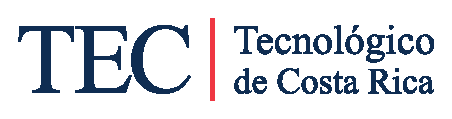
\includegraphics[width=60mm]{Firma_TEC-4}

\par\vspace*{\fill}

{\large\bf{\thesisTitle}}

\par\vspace*{\fill}

Informe de Trabajo Final de Graduación para optar por el título de

Ingeniero en Electrónica con el grado académico de Licenciatura

\par\vspace{20mm}

\thesisAuthor

\vspace*{\fill}

\ifdraft{%
{Borrador de \today}
}{
Cartago, 7 de marzo, 2018
}
\end{center}
\newpage 
\cleardoublepage 


%%% Local Variables: 
%%% mode: latex
%%% TeX-master: "main"
%%% End: 
 % Titlepage in Spanish

  %%% ---------------------------------------------------------------------------
%% titlepage_licce_es.tex
%%
%% Title page
%%
%% $Id: titlepage.tex 1452 2010-07-07 00:55:16Z palvarado $
%% ---------------------------------------------------------------------------

\thispagestyle{empty} 

\begin{center}

Tecnológico de Costa Rica

\par\vspace{1ex}

Área Académica de Ingeniería en Computadores

\par\vspace{1ex}

Programa de Licenciatura de Ingeniería en Computadores

\par\vspace{20mm}

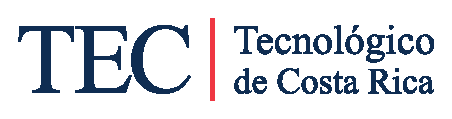
\includegraphics[width=60mm]{Firma_TEC-4}

\par\vspace*{\fill}

{\large\bf{\thesisTitle}}

\par\vspace*{\fill}

Informe de Trabajo Final de Graduación para optar por el título de

Ingeniero en Computadores con el grado académico de Licenciatura

\par\vspace{20mm}

\thesisAuthor

\vspace*{\fill}

\ifdraft{%
{Borrador de \today}
}{
Cartago, 7 de marzo, 2018
}
\end{center}
\newpage 
\cleardoublepage 


%%% Local Variables: 
%%% mode: latex
%%% TeX-master: "main"
%%% End: 
  % Titlepage in Spanish
  %%% ---------------------------------------------------------------------------
%% titlepage_licce_es.tex
%%
%% Title page
%%
%% $Id: titlepage.tex 1452 2010-07-07 00:55:16Z palvarado $
%% ---------------------------------------------------------------------------

\thispagestyle{empty} 

\begin{center}

Tecnológico de Costa Rica

\par\vspace{1ex}

Computer Engineering Department

\par\vspace{1ex}

Licentiate Degree Program in Computer Engineering

\par\vspace{20mm}

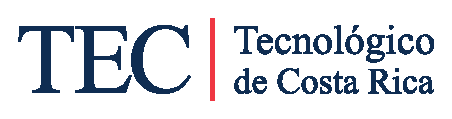
\includegraphics[width=60mm]{Firma_TEC-4}

\par\vspace*{\fill}

{\large\bf{\thesisTitle}}

\par\vspace*{\fill}

Final report submitted in partial fulfillment of the requirements
for the degree of Licentiate in Computer Engineering

\par\vspace{20mm}

\thesisAuthor

\vspace*{\fill}

\ifdraft{%
{Draft \today}
}{
Cartago, March 7th, 2018
}
\end{center}
\newpage 
\cleardoublepage 


%%% Local Variables: 
%%% mode: latex
%%% TeX-master: "main"
%%% End: 
 % Titlepage in English (only if thesis is in En)
  
  %%% ---------------------------------------------------------------------------
%% titlepage_msc_es.tex
%%
%% Title page
%%
%% $Id: titlepage.tex 1452 2010-07-07 00:55:16Z palvarado $
%% ---------------------------------------------------------------------------

\thispagestyle{empty} 

\begin{center}

Tecnológico de Costa Rica

\par\vspace{1ex}

Escuela de Ingeniería Electrónica

\par\vspace{20mm}

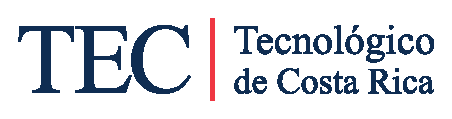
\includegraphics[height=60mm]{Firma_TEC-4}

\par\vspace*{\fill}

{\large\bf{\thesisTitle}}

\par\vspace*{\fill}

Documento de tesis sometido a consideración para optar por el grado
académico de Maestría en Electrónica con Énfasis en
%
%Sistemas Embebidos
Procesamiento Digital de Señales
%Microelectrónica
%Sistemas Microelectromecánicos

\par\vspace{20mm}

\thesisAuthor

\vspace*{\fill}

\ifdraft{%
{Borrador de \today}
}{
Cartago, 19 de noviembre, 2013
}
\end{center}
\newpage 
\cleardoublepage 


%%% Local Variables: 
%%% mode: latex
%%% TeX-master: "main"
%%% End: 
   % Titlepage in Spanish
  %% ---------------------------------------------------------------------------
%% titlepage.tex
%%
%% Title page
%%
%% $Id: titlepage.tex 1452 2010-07-07 00:55:16Z palvarado $
%% ---------------------------------------------------------------------------

\thispagestyle{empty} 

\begin{center}

Tecnológico de Costa Rica

\par\vspace{1ex}

Escuela de Ingeniería Electrónica

\par\vspace{20mm}

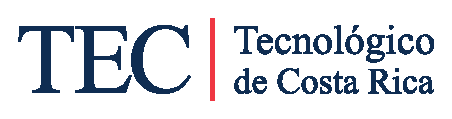
\includegraphics[height=60mm]{Firma_TEC-4}

\par\vspace*{\fill}

{\large\bf{\thesisTitle}}

\par\vspace*{\fill}

A thesis submitted in partial fulfillment of the requirements for the
degree of
%
Master of Science in Electronics, Major in 
%
%Embedded Systems
Digital Signal Processing
%Microelectronics
%Microelectromechanical systems

\par\vspace{20mm}

\thesisAuthor

\vspace*{\fill}

\ifdraft{%
{Draft \today}
}{
Cartago, November 19th, 2017
}
\end{center}
\newpage 
\cleardoublepage 


%%% Local Variables: 
%%% mode: latex
%%% TeX-master: "main"
%%% End: 
   % Titlepage in English (only if thesis is in En)

  \thispagestyle{empty}

\rule{10mm}{0pt}

\vfill

Declaro que el presente documento de tesis ha sido realizado enteramente
por mi persona, utilizando y aplicando literatura referente al tema e
introduciendo conocimientos y resultados experimentales propios.

En los casos en que he utilizado bibliografía he procedido a indicar las
fuentes mediante las respectivas citas bibliográficas.  En consecuencia,
asumo la responsabilidad total por el trabajo de tesis realizado y por
el contenido del presente documento.



\vspace*{8mm}

\begin{flushright}
  \thesisAuthor\par
  Cartago, \today\par
  Céd: 2-0696-0826
\end{flushright}

\cleardoublepage

%%% Local Variables: 
%%% mode: latex
%%% TeX-master: "main"
%%% End: 

  
  %% -------------------------------------------------
  %% Acta y hoja del tribunal
  
  %% Para la licenciatura en electrónica:
  %% ESTE ARCHIVO DEBE ELIMINARSE DE LA VERSIÓN FINAL

\thispagestyle{empty}

\begin{center}
  \begin{tabular}{c}
    Instituto Tecnológico de Costa Rica \\
    Escuela de Ingeniería Electrónica \\
    Proyecto de Graduación \\
    Acta de Aprobación
  \end{tabular}
\end{center}

\vfill

\begin{center}
  \begin{tabular}{c}
    Defensa de Proyecto de Graduación \\
    Requisito para optar por el título de Ingeniero en Electrónica \\
    Grado Académico de Licenciatura
  \end{tabular}
\end{center}

\vfill

%% \thesisAuthorAddress, \thesisAuthor y \thesisTitle están en main.tex
El Tribunal Evaluador aprueba la defensa del proyecto de graduación
denominado \textsl{\thesisTitle}, realizado por
%
\thesisAuthorAddress\ \thesisAuthor\ %
%
y, hace constar que cumple con las normas
establecidas por la Escuela de Ingeniería Electrónica del Instituto
Tecnológico de Costa Rica.

\vfill

\begin{center}
 Miembros del Tribunal Evaluador
\end{center}

\vfill

\begin{center}
  \begin{tabularx}{\textwidth}{cXc}
    \rule{0.45\textwidth}{0.5pt} && \rule{0.45\textwidth}{0.5pt} \\
    \nameLectorI                 && \nameLectorII \\
    \genderLectorI               && \genderLectorII
  \end{tabularx}
  
  \vspace{10mm}

  \begin{tabular}{c}
    \rule{0.45\textwidth}{0.5pt} \\
    \nameAsesor \\
    \genderAsesor
  \end{tabular}
\end{center}

\vfill

\begin{center}
  Cartago, \today\par
\end{center}

\cleardoublepage

%%% Local Variables: 
%%% mode: latex
%%% TeX-master: "main"
%%% End: 
  % Remover en versión final
  %% ESTE ARCHIVO DEBE ELIMINARSE DE LA VERSIÓN FINAL


\thispagestyle{empty}

\begin{center}
  \begin{tabular}{c}
    Instituto Tecnológico de Costa Rica \\
    Escuela de Ingeniería Electrónica \\
    Proyecto de Graduación \\
    Tribunal Evaluador \\
    Acta de Evaluación
  \end{tabular}
\end{center}

\vfill

\begin{center}
  \begin{tabular}{c}
    Defensa de Proyecto de Graduación \\
    Requisito para optar por el título de Ingeniero en Electrónica \\
    Grado Académico de Licenciatura
  \end{tabular}
\end{center}

\vfill

%% \thesisAuthorAddress, \thesisAuthor y \thesisTitle están en main.tex
\begin{center}

  Estudiante:%
  \qquad \textbf{\thesisAuthor}%
  \qquad Carné: \thesisAuthorTECID

  \vspace*{2ex}

  \setlength\tabcolsep{0pt}
  \begin{tabular}{p{.25\textwidth}p{.73\textwidth}}
    Nombre del proyecto: & \textsl{\thesisTitle}
  \end{tabular}
\end{center}
\vspace{5mm}

\vfill

Los miembros de este Tribunal hacen constar que este proyecto de
graduación ha sido aprobado y cumple con las normas establecidas por
la Escuela de Ingeniería Electrónica del Instituto Tecnológico de
Costa Rica y es merecedor de la siguiente calificación:

\vfill

\begin{center}
  Nota de Proyecto de Graduación: \rule{25mm}{0.5pt}
\end{center}

\vfill

\begin{center}
 Miembros del Tribunal Evaluador
\end{center}

\vfill

% Defina con \setLector* en main.tex los lectores y asesor
\begin{center}
  \begin{tabularx}{\textwidth}{cXc}
    \rule{0.45\textwidth}{0.5pt} && \rule{0.45\textwidth}{0.5pt} \\
    \nameLectorI                 && \nameLectorII \\
    \genderLectorI               && \genderLectorII
  \end{tabularx}
  
  \vspace{10mm}

  \begin{tabular}{c}
    \rule{0.45\textwidth}{0.5pt} \\
    \nameAsesor \\
    \genderAsesor
  \end{tabular}
\end{center}

\vfill

\begin{center}
  Cartago, \today\par
\end{center}

\cleardoublepage

%%% Local Variables: 
%%% mode: latex
%%% TeX-master: "main"
%%% End: 
      % Remover en versión final
  
  %% Para la maestría en electrónica:
  %%% ESTE ARCHIVO DEBE ELIMINARSE DE LA VERSIÓN FINAL

\thispagestyle{empty}

\begin{center}
  \begin{tabular}{c}
    Instituto Tecnológico de Costa Rica \\
    Escuela de Ingeniería Electrónica \\
    Proyecto de Graduación \\
    Tesis de Maestría \\
    Tribunal Evaluador
  \end{tabular}
\end{center}

\vfill

Tesis de maestría defendida ante el presente Tribunal Evaluador como
requisito para optar por el grado académico de maestría, del Instituto
Tecnológico de Costa Rica.

\vfill

\vspace*{20mm}
\begin{center}
 Miembros del Tribunal
\end{center}
\vspace*{8mm}

\vfill

\begin{center}
  \begin{tabularx}{\textwidth}{cXc}
    \rule{0.45\textwidth}{0.5pt} && \rule{0.45\textwidth}{0.5pt} \\
    \nameLectorI                 && \nameLectorII \\
    \genderLectorI               && \genderLectorII
  \end{tabularx}
  
  \vspace{10mm}

  \begin{tabular}{c}
    \rule{0.45\textwidth}{0.5pt} \\
    \nameAsesor \\
    \genderAsesor
  \end{tabular}
\end{center}

\vfill


Los miembros de este Tribunal dan fe de que la presente tesis de maestría 
ha sido aprobada y cumple con las normas establecidas por la Escuela de
Ingeniería Electrónica.

\vfill

\begin{center}
  Cartago, \today\par
\end{center}

\cleardoublepage

%%% Local Variables: 
%%% mode: latex
%%% TeX-master: "main"
%%% End: 
  % Remover en versión final
  %%% ESTE ARCHIVO DEBE ELIMINARSE DE LA VERSIÓN FINAL


\thispagestyle{empty}

\begin{center}
  \begin{tabular}{c}
    Instituto Tecnológico de Costa Rica \\
    Escuela de Ingeniería Electrónica \\
    Tesis de Maestría \\
    Acta de Evaluación
  \end{tabular}
\end{center}

\vfill

Tesis de maestría defendida ante el presente Tribunal Evaluador como
requisito para optar por el grado académico de maestría, del Instituto
Tecnológico de Costa Rica.

\vspace*{15mm}

%% Definir \thesisAuthor, \thesisTitle, etc. en archivo main.tex
\begin{center}
  Estudiante: \thesisAuthor
\end{center}

\vfill

\begin{center}
  Nombre del Proyecto: \thesisTitle}
\end{center}

\vspace*{20mm}
\begin{center}
 Miembros del Tribunal Evaluador
\end{center}
\vspace*{8mm}

\vfill

% Los nombres de lectores y asesor se definen en el archivo main.tex
\begin{center}
  \begin{tabularx}{\textwidth}{cXc}
    \rule{0.45\textwidth}{0.5pt} && \rule{0.45\textwidth}{0.5pt} \\
    \nameLectorI                 && \nameLectorII \\
    \genderLectorI               && \genderLectorII
  \end{tabularx}
  
  \vspace{10mm}

  \begin{tabular}{c}
    \rule{0.45\textwidth}{0.5pt} \\
    \nameAsesor \\
    \genderAsesor
  \end{tabular}
\end{center}

\vfill

Los miembros de este Tribunal dan fe de que la presente tesis de
maestría ha sido aprobada y cumple con las normas establecidas por la
Escuela de Ingeniería Electrónica.

\vfill

\begin{center}
  Nota final de la Tesis de Maestría: \rule{3cm}{0.5pt}
\end{center}
\vfill

\begin{center}
  Cartago, \today\par
\end{center}

\cleardoublepage

%%% Local Variables: 
%%% mode: latex
%%% TeX-master: "main"
%%% End: 
      % Remover en versión final
  %% -------------------------------------------------
  
  \chapter*{Resumen}
\thispagestyle{empty}

El resumen es la síntesis de lo que aparecerá en el tesis. Tiene que ser lo
suficientemente consiso y claro para que alguien que lo lea sepa qué esperar
del resto de la tesis si la leyera completamente. Puede concluir con palabras
clave, que son los temas principales tratados en el documento. El resumen queda
fuera de la numeración del resto de secciones.

No se acostumbra utilizar referencias bibliográficas, tablas, o figuras
en el resumen.

\bigskip

\textbf{Palabras clave:} \thesisKeywords

\clearpage
\chapter*{Abstract}
\thispagestyle{empty}

The same as before, but in English.

\bigskip

\textbf{Keywords:} word 1, word 2, 

\cleardoublepage

%%% Local Variables: 
%%% mode: latex
%%% TeX-master: "main"
%%% End: 

  \vspace*{0.4\textheight}
{\hfill{\Large{\emph{a Mariángel}}}}

  \chapter*{Agradecimientos}
\thispagestyle{empty}

El resultado de este trabajo no hubiese sido posible sin el apoyo de Thevenin,
Norton, Einstein y mi querido amigo Ohm.

\vspace*{1cm}

\thesisAuthor

Cartago, \today

\cleardoublepage

%%% Local Variables: 
%%% mode: latex
%%% TeX-master: "paMain"
%%% End: 


  %----------------------------------------------------------------------------
  \frontmatter
  %----------------------------------------------------------------------------
  \pagestyle{fancy}
  \pagenumbering{roman}

  \pdfbookmark[1]{Indice General}{Indice General}

  \parskip0ex                           % space between paragraphs

  \tableofcontents                      % Table of contents
  \listoffigures                        % List of figures
  \listoftables                         % List of tables

\ifdraft{%
  % todo's                              % TODOs
  \listoftodo
}{%
}

  %% ---------------------------------------------------------------------------
%% paNotation.tex
%%
%% Notation
%%
%% $Id: notation.tex 1467 2010-07-24 16:47:17Z palvarado $
%% ---------------------------------------------------------------------------

\newcommand{\nms}{\negmedspace}

%%
% Commands required for the nomenclature groups
%
% There are following prefix forms:
%  a   abbreviation    \syma[key]{symbol}{description}
%  g   general         \symg[key]{symbol}{description}
%%

\newcommand{\nmstyle}[1]{\large\item[\textbf{#1}]\normalsize}

\renewcommand{\nomgroup}[1]{%
  \ifthenelse{\equal{#1}{A}}{\nmstyle{Abbreviations}\normalsize}{%
  \ifthenelse{\equal{#1}{G}}{\bigskip\nmstyle{General notation}\normalsize}%
  }
}

\newcommand{\syma}[3][foo]{%
  \ifthenelse{\equal{#1}{foo}}%
  {\nomenclature[A#2\ ]{#2}{#3}}{\nomenclature[A#1\ ]{#2}{#3}}}
\newcommand{\symg}[3][foo]{%
  \ifthenelse{\equal{#1}{foo}}%
  {\nomenclature[G#2\ ]{#2}{#3}}{\nomenclature[G#1\ ]{#2}{#3}}}

%%
% Command definitions for localized symbol format definition
%%
\renewcommand{\Re}{\operatorname{Re}}
\renewcommand{\Im}{\operatorname{Im}}

\newcommand{\prt}[1]{\ensuremath{\mathcal{#1}}}         %% partitioning
\newcommand{\img}[1]{\ensuremath{\mathcal{#1}}}         %% image as a set
\newcommand{\reg}[1][R]{\ensuremath{\mathcal{#1}}}      %% region
\newcommand{\pred}[1]{\ensuremath{\mathrm{#1}}}         %% predicate
\newcommand{\operat}[2]{\mathcal{#1}\left\{#2\right\}}
\newcommand{\transf}[1]{\mathscr{#1}}
\newcommand{\fourier}[1]{\transf{F}\left\{#1\right\}}
\newcommand{\ifourier}[1]{\transf{F}^{-1}\left\{#1\right\}}
\newcommand{\laplace}[1]{\transf{L}\left\{#1\right\}}
\newcommand{\ulaplace}[1]{\transf{L}_u\left\{#1\right\}}
\newcommand{\blaplace}[1]{\transf{L}_b\left\{#1\right\}}
\newcommand{\ilaplace}[1]{\transf{L}^{-1}\left\{#1\right\}}
\newcommand{\ztrans}[1]{\transf{Z}\left\{#1\right\}}
\newcommand{\iztrans}[1]{\transf{Z}^{-1}\left\{#1\right\}}
\newcommand{\zutrans}[1]{\transf{Z}_u\left\{#1\right\}}
\newcommand{\exceq}{\ensuremath{\overset{!}{=}}}

\newcommand{\signum}{\operatorname{signum}}
\newcommand{\vct}[1]{\ensuremath{\underline{\mathbf{#1}}}}
\newcommand{\mat}[1]{\ensuremath{\mathbf{#1}}}
\newcommand{\vctmu}{\vct{\boldsymbol{\mu}}}
\newcommand{\vctzeta}{\vct{\boldsymbol{\zeta}}}
\newcommand{\vctpi}{\vct{\boldsymbol{\pi}}}
\newcommand{\vctvarphi}{\vct{\boldsymbol{\varphi}}}
\newcommand{\raum}[1]{\ensuremath{\mathbb{#1}}}
\newcommand{\matSigma}{\mat{\boldsymbol{\Sigma}}}
\newcommand{\matLambda}{\mat{\boldsymbol{\Lambda}}}
\newcommand{\matPsi}{\mat{\boldsymbol{\Psi}}}
\newcommand{\matPhi}{\mat{\boldsymbol{\Phi}}}
\newcommand{\row}[2]{\ensuremath{\mathbf{\underline{#1}_{#2(\cdot)}}}}
\newcommand{\col}[2]{\ensuremath{\mathbf{\underline{#1}_{(\cdot) #2}}}}
\newcommand{\seq}[1]{\ensuremath{#1}}
\newcommand{\set}[1]{\ensuremath{\mathcal{#1}}}
\newcommand{\gset}[1]{\ensuremath{#1}} %% set for greek symbols
\newcommand{\front}[1]{\widehat{\set{#1}}}
\newcommand{\setlambda}{\set{\boldsymbol{\lambda}}}
\newcommand{\klass}[1]{\ensuremath{\mathpss{#1}}}
\newcommand{\graph}[1]{\ensuremath{\mathsf{#1}}}
\newcommand{\lab}[1]{\ensuremath{\mathpss{L}(#1)}}
\newcommand{\myfrac}[2]{{\footnotesize #1/#2}}
\newcommand{\ifthenspc}{\rule{3mm}{0mm}}
\newcommand{\point}[1]{\ensuremath{\mathsf{#1}}}
\newcommand{\estim}[1]{\ensuremath{\hat{#1}}}
\newcommand{\numset}[1]{\ensuremath{\mathbb{#1}}}
\newcommand{\tuple}[1]{\ensuremath{\left\langle#1\right\rangle}}
\newcommand{\norm}[1]{\ensuremath{\left\lVert#1\right\rVert}}
\newcommand{\conj}[1]{\ensuremath{{{#1}^{\ast}}}}
\newcommand{\base}[1]{\set{#1}}
\newcommand{\zeron}[1]{\ensuremath{\underset{\uparrow}{#1}}}
\newcommand{\sysT}{\ensuremath{\mathcal{T}}}
\newcommand{\sys}[1]{\ensuremath{\sysT\left[#1\right]}}
%\newcommand{\sen}{\operatorname{sen}} % sinus in spanish (seno)
%\newcommand{\senh}{\operatorname{senh}} % sinus hiperbolicus in spanish (seno)
%\newcommand{\arcsen}{\operatorname{arcsen}} % arcus sinus hiperbolicus in spanish (arcoseno)
\newcommand{\sgn}{\operatorname{sgn}} % signus
\newcommand{\roc}{\text{ROC: }}

\newcommand{\code}[1]{\texttt{#1}}
\newcommand{\conv}{\ensuremath{\ast}}
\newcommand{\cconv}{\ensuremath{\;\,\text{\footnotesize{N}}\!\!\!\!\!\!\bigcirc}}
\newcommand{\Ln}{\operatorname{Ln}}
\newcommand{\rand}{\operatorname{rand}}
\newcommand{\sa}{\operatorname{sa}}
\newcommand{\senc}{\operatorname{senc}}
\newcommand{\si}{\operatorname{si}}


%% Natural, Integer and Real Numbers
\newcommand{\setA}{\ensuremath{\mathbb{A}}}
\newcommand{\setB}{\ensuremath{\mathrm{I\negthinspace B}}}
\newcommand{\setC}{\ensuremath{\mathbb{C}}}
\newcommand{\setD}{\ensuremath{\mathrm{I\negthinspace D}}}
\newcommand{\setE}{\ensuremath{\mathrm{I\negthinspace E}}}
\newcommand{\setF}{\ensuremath{\mathrm{I\negthinspace F}}}
\newcommand{\setG}{\ensuremath{\mathbb{G}}}
\newcommand{\setH}{\ensuremath{\mathrm{I\negthinspace H}}}
\newcommand{\setI}{\ensuremath{\mathbb{I}}}
\newcommand{\setJ}{\ensuremath{\mathbb{J}}}
\newcommand{\setK}{\ensuremath{\mathrm{I\negthinspace K}}}
\newcommand{\setL}{\ensuremath{\mathrm{I\negthinspace L}}}
\newcommand{\setM}{\ensuremath{\mathrm{I\negthinspace M}}}
\newcommand{\setN}{\ensuremath{\mathrm{I\negthinspace N}}}
\newcommand{\setO}{\ensuremath{\mathbb{O}}}
\newcommand{\setP}{\ensuremath{\mathrm{I\negthinspace P}}}
\newcommand{\setQ}{\ensuremath{\mathbb{Q}}}
\newcommand{\setR}{\ensuremath{\mathrm{I\negthinspace R}}}
\newcommand{\setS}{\ensuremath{\mathbb{S}}}
\newcommand{\setT}{\ensuremath{\mathbb{T}}}
\newcommand{\setU}{\ensuremath{\mathbb{U}}}
\newcommand{\setV}{\ensuremath{\mathbb{V}}}
\newcommand{\setW}{\ensuremath{\mathbb{W}}}
\newcommand{\setX}{\ensuremath{\mathbb{X}}}
\newcommand{\setY}{\ensuremath{\mathbb{Y}}}
\newcommand{\setZ}{\ensuremath{\mathbb{Z}}}


%%
% Multimap symbols
%
\newcommand{\ttoF}{\,\circ\!\negthickspace\longrightarrow\negthickspace\!\negthickspace\bullet\,}
\newcommand{\Ftot}{\,\bullet\negthickspace\!\negthickspace\longleftarrow\!\negthickspace\circ\,}
\newcommand{\ttoZ}{\ttoF}
\newcommand{\Ztot}{\Ftot}
\newcommand{\ttoZu}{\overset{z_u}{\ttoF}}
\newcommand{\Zutot}{\overset{z_u}{\Ftot}}
\newcommand{\vttoF}{\text{\begin{sideways}$\Ftot$\end{sideways}}}
\newcommand{\vFtot}{\text{\begin{sideways}$\ttoF$\end{sideways}}}
\newcommand{\vttoZ}{\vttoF}
\newcommand{\vZtot}{\vFtot}
\newcommand{\ttoDF}{\underset{N}{\ttoF}}
\newcommand{\DFtot}{\underset{N}{\Ftot}}

\newcommand{\thisis}[2]{\underset{#1}{\underbrace{#2}}}

%%% Local Variables:
%%% mode: latex
%%% TeX-master: "paMain"
%%% End:
                    % Notation
  %% ---------------------------------------------------------------------------
%% paNotation.tex
%%
%% Notation
%%
%% $Id: paNotation.tex,v 1.15 2004/03/30 05:55:59 alvarado Exp $
%% ---------------------------------------------------------------------------

\cleardoublepage
\renewcommand{\nomname}{List of symbols and abbreviations}
\markboth{\nomname}{\nomname}
\renewcommand{\nompreamble}{\addcontentsline{toc}{chapter}{\nomname}%
\setlength{\nomitemsep}{-\parsep}
\setlength{\itemsep}{10ex}
}

%%
% Símbolos en la notación general
% (es posible poner la declaración en el texto
%%

\symg[t]{$\sys{\cdot}$}{Transformation performed by a system}
\symg[yscalar]{$y$}{Scalar.}
\symg[zconjugado]{$\conj{z}$}{Conjugate Complex of $z$}
\symg[rcomplexreal]{$\Re(z)$ o $z_{\Re}$}{Real part of the complex number $z$}
\symg[icompleximag]{$\Im(z)$ o $z_{\Im}$}{Imaginary part of the complex number $z$}
\symg[jimaginario]{$j$}{$j=\sqrt{-1}$}
\symg[xvector]{$\vct{x}$}{Vector. \newline\hspace{1mm}%
  $\vct{x}=\left[ x_1 \; x_2 \; \ldots \; x_n \right]^T =
  \begin{bmatrix}
    x_1 \\ x_2 \\ \vdots \\ x_n
  \end{bmatrix}$}

\symg[amatrix]{$\mat{A}$}{Matrix. \newline\hspace{1mm}%
  $\mat{A} =
  \begin{bmatrix}
    a_{11} & a_{12} & \cdots & a_{1m}\\
    a_{21} & a_{22} & \cdots & a_{2m}\\
    \vdots & \vdots & \ddots & \vdots\\
    a_{n1} & a_{n2} & \cdots & a_{nm}\\
  \end{bmatrix}$}

\symg[C]{$\setC$}{Complex numbers set.}

%%
% Algunas abreviaciones
%%

\syma{MLP}{Multilayer perceptrons}
\syma{CNN}{Convolutional Neural Networks}
\syma{VAE}{Variational Autoencoder}
\syma{sVAE}{Spatial Variational Autoencoder}
\syma{GM-VAE}{Gaussian-Mixture Variational Autoencoder}
\syma{GAN}{Generative Adversarial Networks}
\syma{KL}{Kullback-Leibler}
\syma{MVN}{Matrix-variable normal distribution}

\printnomenclature[20mm]

%%% Local Variables:
%%% mode: latex
%%% TeX-master: "paMain"
%%% End:
                    % Abbreviation

  \parskip1.3ex                         % space between paragraphs

  %----------------------------------------------------------------------------
  \mainmatter
  %----------------------------------------------------------------------------
  % where to look for graphics
  \graphicspath{{./}{./fig/}}
  %\pagenumbering{arab}

  % Main files
  %% ---------------------------------------------------------------------------
%% intro.tex
%%
%% Introduction
%%
%% $Id: intro.tex 1477 2010-07-28 21:34:43Z palvarado $
%% ---------------------------------------------------------------------------

\chapter{Introducción}
\label{chp:intro}

En la \nt{introducción} deben quedar completamente claros los siguientes
aspectos, cuyo significado depende del tipo concreto de tesis:

\begin{compactitem}
\item Contexto
\item Problema
\item Esbozo de solución
\item Objetivos y estructura
\end{compactitem}

El contexto corresponde al entorno donde se desarrolla el proyecto de
tesis, que puede ser el área general de aplicación, un dominio de
problemas, etc. El problema concreto se sintetiza usualmente en una
frase o pregunta. Esta pregunta debería ser una consecuencia a la que
se llega después de realizar el desarrollo del contexto. Del
planteamiento del problema se deriva cuál es el objetivo del trabajo
en particular, que a su vez debe conducir al lector de forma natural
al esbozo de la solución del problema a tratar en la
tesis. Generalmente para aclarar la solución se hace uso de un
diagrama de bloques o diagrama de flujo general, es decir, desde un
nivel de abstracción alto, donde no sea necesario entrar en detalles
técnicos. Usualmente este diagrama y su breve explicación dictan cuál
debe ser la estructura del resto del tesis, que es mencionada siempre
al final de la introducción.

Una buena introducción debe lograr que el lector tenga interés de leer el resto
del tesis.

Es recomendable dividir la tesis en secciones, nombradas cada una de acuerdo a
su contenido. \textbf{Jamás} utilice los nombres de la guía como
``\emph{Problema existente e importancia de su solución}'', sino algo como ``La
deforestación en Costa Rica'' o lo que se adecúe a su problema en particular.

Recuerde que en español solo la primera letra del título va en mayúscula
(exceptuando nombres propios, por supuesto).

\section{Objetivos y estructura del documento}

\index{objetivos}
Esta plantilla LaTeX tiene como objetivo simplificar la construcción del
documento de tesis, presentando ejemplo de figuras y tablas, así como otorgar
una plataforma de compilación en GNU/Linux que simplifique la administración de
todo el documento.

La última sección de la introducción usualmente sí tiene un título estandar que
es ``Objetivos y estructura del documento'', donde se presentan \emph{en prosa}
los objetivos general y específicos que ha tenido el proyecto de tesis,
así como la estructura de la tesis (por ejemplo, ``en el siguiente capítulo se
esbozan los fundamentos teóricos necesarios para explicar en el
capítulo~\ref{ch:solucion} la propuesta realizada$\ldots$''

%%% Local Variables: 
%%% mode: latex
%%% TeX-master: "main"
%%% End: 

  \chapter{Marco teórico}
\label{ch:marco}

\section{Descripción}

Toda tesis hace referencia a trabajos previos en el área y trabajos afines que
están directamente relacionados con lo planteado en el tesis.

Además, en el marco teórico debe aparecer la información absolutamente
necesaria para comprender la solución, y por eso es recomendable escribir
primero la solución (el siguiente capítulo), para ir anotando qué debe ser
explicado en el marco teórico.

\section{Generalidades}

Se recomienda revisar las guías de publicación de la \nt{IEEE} en
\url{http://www.ieee.org/publications_standards/publications/authors/authors_journals.html},
donde puede encontrar cómo hacer referencias bibliográficas correctamente, cómo
citar ecuaciones, tablas y figuras, etc.  

\subsection{Redacción}

La \nt{redacción} en todo el documento debe seguir un estilo científico
objetivo. Esto implica que se redacta de modo impersonal, sin utilizar primeras
personas del singular o del plural, y se evita el uso de cualquier tipo de
calificativo, sustituyéndolos siempre por datos concretos, vinculados a
referencias bibliográficas o datos experimentales. Los comparativos también
deben concretarse a hechos y datos, y nunca dejarse ``en el aire''. Por la
naturaleza de la tesis, el tiempo verbal es usualmente presente, no perdiendo
nunca de vista que se está explicando ``cómo hacer algo'', en vez de ``qué se
hizo''.

Las \nt{frases} deben ser cortas, y debe evitarse que el lector tenga que saltar
constantemente entre partes de la tesis, lo que implica una exposición lineal
clara, donde lo que se necesita ya ha sido explicado antes. Deben evitarse
redundancias y por tanto cada concepto se exponen en un único lugar.

Todo aspecto circunstancial es irrelevante para la tesis, es decir, si se ha
desarrollado en el laboratorio $X$, o en el curso $Y$, con el profesor $Z$, o
en la empresa $W$, el nombre de funciones o clases en su código, etc., es
información irrelevante para reproducir el experimento, y por lo tanto sobra.
%
Esa información puede incluirse en uno de los anexos.


\subsubsection{Numeración del documento}

La primera página de la tesis es la correspondiente a la introducción,
así que ésta debe ser la página 1. Desde la introducción, hasta antes
de la bibliografía, las unidades son ``Capítulos''. La bibliografía y
anexos no se consideran capítulos, así que ya no continúan con la
misma numeración de los capítulos (la paginación sí continua). Los
índices, notación, glosario, etc.\ se numeran con números romanos en
versalitas ({\textsc{I}, \textsc{II}, \textsc{III}, \textsc{IV},
  \textsc{V}, \textsc{VI}}$\ldots$) y antes del índice (portada,
resúmenes, agradecimientos, hoja de evaluadores, etc.) las páginas no
llevan numeración.

Esta plantilla LaTeX ya se ocupa de todo lo anterior.

\subsection{Ecuaciones}

Para citar \nt{ecuaciones} se utilizan paréntesis redondos, y no es
necesario emplear explícitamente la palabra ``ecuación''. Por ejemplo
``Introduciendo en (4.2) los resultados de (3.3) y (3.7) se obtiene
...''. La ecuación es parte del flujo de texto y no un objeto
flotante, así que no pueden emplearse como figuras. Cuando se requiere
la ecuación, allí se inserta.

Es incorrecto redactar de la siguiente forma: \explain{MAL}

\textsl{La operación del transistor sin tomar en cuenta el efecto Early está
  dada por (\ref{eq:ej1}), donde el parámetro $\kappa$ está dado por
  (\ref{eq:ej2}).}

\begin{equation} \label{eq:ej1}
  I_{DS}
  =
  I_{n0} \frac{W}{L}e^{\kappa \frac{V_{GB}}{v_t}}
  \left[
    e^{-\frac{V_{SB}}{v_t}}
    -
    e^{-\frac{V_{DB}}{v_t}}
  \right]
\end{equation}

\begin{equation} \label{eq:ej2}
  \kappa = \frac{C_{ox}}{C_{ox}+C_{dep}}
\end{equation}

Lo anterior es incorrecto porque obliga al lector a estar buscando ecuaciones,
que pueden mostrarse directamente.  La única referenciación permitida es hacia
atrás.

La forma correcta de redactar lo anterior es: \chk{BIEN}

\textsl{La operación del transistor sin tomar en cuenta el efecto Early está
  dada por}
\begin{equation} \label{eq:ej3}
  I_{DS}
  =
  I_{n0} \frac{W}{L}e^{\kappa \frac{V_{GB}}{v_t}}
  \left[
    e^{-\frac{V_{SB}}{v_t}}
    -
    e^{-\frac{V_{DB}}{v_t}}
  \right]
\end{equation}
\textsl{donde el parámetro $\kappa$ es}
\begin{equation} \label{eq:ej4}
  \kappa = \frac{C_{ox}}{C_{ox}+C_{dep}}
\end{equation}

Así el flujo del texto guía al lector por las ecuaciones sin mayor esfuerzo.

Es recomendable numerar \emph{todas} las ecuaciones, de modo que en la revisión
del documento, o en futuras referencias a su documento de tesis todas las
ecuaciones puedan ser citadas sin requerir describir textualmente a cuál
ecuación se está haciendo referencia.

Es preferible utilizar coma decimal en vez de punto decimal, debido a
que es el estándar internacional.  El Diccionario panhispánico de
dudas aclara que se acepta el punto como separador decimal, pero eso
no quiere decir que sea preferible.  Esta plantilla ya incorpora el
uso del paquete de \LaTeX\ \code{icomma}, que se encarga de realizar
el espaciado correcto de la coma.  Cuando utilice coma como signo de
puntuación, deje un espacio posterior, para asegurarse de que
\code{icomma} no lo tome como separador decimal.

\begin{equation}
  \label{eq:normrnd}
  h(x)=\norm{\rand()-0,5}^2_2
\end{equation}

\subsection{Figuras}

Para el almacenamiento de imágenes existen dos tipos de formato: las imágenes
raster y las imágenes vectoriales.\index{imagen!raster}

\subsubsection{Imágenes raster}

Las imágenes raster son representadas por una rejilla de píxeles, en donde cada
píxel tiene un valor que representa al nivel de gris o el color. La
discretización espacial es ineludible, y la única forma de obtener buena
calidad es empleando tamaños grandes de la imagen que conduzcan a resoluciones
de al menos 300 puntos por pulgada en la impresión, lo que conlleva a archivos
de documentos de varios megabytes. Dentro de los formatos para almacenar
imágenes raster existen algunos con pérdida (como el JPEG) que producen en
imágenes sintéticas, como diagramas, estructuras ruidosas que dan una
apariencia de baja calidad a las figuras. Otros formatos (como PNG, BMP, TIFF o
GIF) no tiene pérdidas de información, pero los algoritmos de compresión no
pueden reducir el tamaño de las imágenes con los mismos factores de reducción
que los formatos con pérdidas. Este tipo de formatos debe utilizarse únicamente
para fotografías o capturas de escenas reales con cámaras digitales.

\subsubsection{Imágenes vectoriales}

\index{imagen!vectorial}
Las imágenes vectoriales \textbf{deben} ser empleadas en todo tipo de
diagrama. En ellas no se almacenan píxeles, sino las estructuras geométricas
que componen la figura como círculos (representado por posicion de su centro y
su radio), rectángulos (representados por sus esquinas), líneas, texto, etc. La
mayoría de programas para elaborar este tipo de diagramas, como Inkscape, XFig,
OpenOffice.org Draw, MS Visio, Adobe Illustrator, etc. proveen varios formatos
vectoriales que pueden ser insertados tanto en LaTeX como en OpenOffice.org
Writer (o MS Word). Los formatos más empleados son los llamados metafiles, que
incluyen al WMF, EMF. En LaTeX se utiliza por lo general EPS. Recientemente se
ha incrementado el soporte al formato SVG.

No debe cometerse el error de generar una imagen vectorial a partir de una
imagen raster, pues una vez realizada la discretización espacial no es posible
reconstruir los elementos geométricos que componen la imagen. Por ello, no
tiene ningún sentido generar un archivo EPS o WMF a partir de una imagen ya
almacenada en BMP, JPG, o PNG, pues lo único que ocurrirá es que se inserta la
figura raster tal cual en la imagen vectorial, sin implicar ninguna ganancia en
la calidad.

Esta plantilla de LaTeX administra la generación de ciertas figuras por usted.
Puede colocar en el directorio \texttt{fig/} archivos EPS, JPG, PNG o GP (de
GNUPlot) y el Makefile se encarga de hacer todas las conversiones necesarias.
En las siguientes subsecciones se describen dos casos adicionales que resultan
útiles para realizar figuras más complejas.

\subsubsection{Figuras tikz}
\index{tikz}

Esta plantilla compila archivos con código en Tikz para generar
figuras.
%
En realidad, lo único que hace el Makefile es compilar con
\code{pdflatex} cualquier archivo \texttt{fig/*.tikz} y dejar el
resultado en el directorio de figuras, aunque el concepto fue pensado
particularmente para generar imágenes vectoriales utilizando las
características de Tikz, biblioteca de LaTeX que es utilizada cada vez
más por su enorme flexibilidad.
%
\begin{figure}[htb]
  \centering
  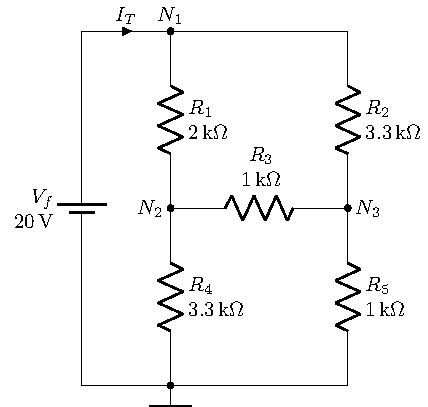
\includegraphics{figtemplate}
  \caption[Ejemplo de figura con tikz]{Ejemplo realizado con
    \texttt{tikz}.  Usted encuentra la plantilla en el directorio de
    figuras bajo el nombre \texttt{fig/figtemplate.tikz}.}
  \label{fig:figtemplate}
\end{figure}

La figura~\ref{fig:figtemplate} muestra un ejemplo que se puede
utilizar como plantilla para generar figuras \texttt{tikz}.  La
plantilla la encuentra en el directorio de figuras y se llama
\code{figtemplate.tikz}.


\subsubsection{Figuras ltxfig/psfrag}

\index{psfrag}\index{ltxfig}
Cuando en el subdirectorio \texttt{fig/} se encuentran dos archivos con el
mismo nombre pero extensiones \texttt{ltxfig} y \texttt{psfrag}, por ejemplo
\texttt{prueba.ltxfig} y \texttt{prueba.psfrag}, entonces el Makefile asume que
usted desea crear una figura a partir del archivo \texttt{prueba.ltxfig},
creado con el programa \texttt{XFig}, sustituyendo los textos ahí presentes con
texto formateado con LaTeX.

La figura~\ref{fig:ltxfig} ha sido creada con este esquema.  Revise los
archivos correspondientes en el directorio de figuras
\texttt{fig/ltxfig\_prototipo.*} para más detalles sobre su uso.

\begin{figure}[htb]
  \centering
  \includegraphics[width=0.9\textwidth]{ltxfig_prototipo}
  \caption{Ejemplo de imagen ltxfig/psfrag}
  \label{fig:ltxfig}
\end{figure}

\subsubsection{Figuras pstricks}  

\index{pstricks}
Los archivos con extensión \texttt{.pstricks} en el directorio \texttt{fig} se
utilizan para generar cualquier tipo de imágenes según el código que se
contenga.  Es un concepto más general que el anterior.  La
figura~\ref{fig:pstricks} ha sido creada con este esquema.  Puede revisar los
archivos \texttt{prototipo\_gnuplot*} como un ejemplo de su uso, en donde de un
archivo gnuplot (\texttt{\_.gp}) se genera un archivo \texttt{\_.eps}, el cual
es incluido en el archivo \texttt{.pstricks} sustituyendo cadenas de texto por
código LaTeX.

\begin{figure}[htb]
  \centering
  \includegraphics{prototipo_gnuplot}
  \caption{Ejemplo de imagen gnuplot/pstricks}
  \label{fig:pstricks}
\end{figure}



\subsubsection{Entradas en el índice de figuras}

El índice de figuras debe servir para encontrar rápidamente dónde se
encuentra cierta figura.  El pie de la figura, indicado en \LaTeX con
\texttt{caption} puede ser extenso, en especial para indicar detalles
de las figura, y es la entrada por defecto que aparecerá en el índice
de figuras, la cual no debe superar la extensión de una línea y debe
únicamente dar la idea del contenido de la figura para poder ser
encontrada.  Para lograr esto en \LaTeX{} se agrega un parámetro
opcional con el texto del índice de la siguiente forma:
\begin{verbatim}
  \caption[Texto en el índice]{Texto al pie de la figura}
\end{verbatim}

\subsection{Referencias bibliográficas}

\index{referencias}\index{BibTeX}
Todo concepto o idea tomado de otros autores contar con la respectiva
referencia. En redacción técnica de ingeniería rara vez se utiliza la cita
textual, así que es necesario reformular las ideas y conceptos con palabras
propias. En ingeniería electrónica se utilizan los formatos de referencia de la
IEEE o la ACM, que son numéricos, encerrados entre paréntesis cuadrados (por
ejemplo, ``En \cite{Davis1963} se propuso un nuevo algoritmo'', o ``En
\cite{ProakisManolakis1998} los autores proponen tomar las ventajas de los
algorimos presentados en \cite{Oppenheim1998,Roberts2005,Haykin2001} por medio
del método de Newton \cite{Burrus1998} conocido en el área de optimización
lineal.''). La referencia es parte de las frases, así que si la frase termina
con la referencia para indicar la idea, ésta debe estar antes del punto final o
demás signos de puntuación: ``La capacidad de memoria también sigue una Ley
similar a la de Moore \cite{Octave}. Los siguientes son los aspectos a tomar en
cuenta en el diseño del sistema \cite{Lindner2002}:''

Se recomienda utilizar BibTeX para indicar las referencias
bibliográficas.  Actualmente herramientas como Mendeley, Zotero u
otras similares simplifican la administración de las referencias y
pueden exportar al formato BibTeX.

\subsection{Extensión}

\index{extensión}
Una tesis de licenciatura no debe sobrepasar las 120 páginas incluyendo
apéndices y los formalismos desde portada hasta índices.

El cuerpo de la tesis (desde introducción hasta conclusiones) usualmente se
extiende desde 45 páginas hasta no más de 80, dependiendo de la problemática
tratada.

No es necesario reproducir contenidos de otras fuentes: agregue las referencias
a dichas fuentes, y limítese a enunciar lo estrictamente necesario para
comprender sus propuestas de solución.

\section{Sobre esta plantilla \LaTeX}

Esta plantilla \LaTeX pretende simplificar varios pasos en la creación del
documento de tesis.

\subsection{Marcar asuntos pendientes}

La plantilla tiene dos ``\emph{modos}'' de operación: normal y borrador
(\emph{draft}).  En el archivo \texttt{main.tex} a partir de la línea 41 usted
encuentra el código

\begin{verbatim}
%
% DRAFT MODE
%
\newboolean{draftmode}                  % boolean used to control draft-mode
% Ensure that only one of the next two lines is active:
\setboolean{draftmode}{true}            % turn draft mode on
%\setboolean{draftmode}{false}           % turn draft mode off
\end{verbatim}

Con el modo borrador, se activan ciertos comandos y funcionalidades útiles en
el proceso de elaboración de la tesis, pero que deben ser desactivados al
final, antes de entregar la tesis.  Por ejemplo, se activa el pie de página que
dice ``\emph{Borrador: fecha}'', y se activa el índice titulado ``Revisar''.  En dicho índice aparecen las páginas en donde se hayan utilizado alguno de los siguientes comandos:
\begin{compactitem}
\item \verb+\boxcomment{comentario}+ Crea una caja en el margen de página con
  el comentario indicado.
\item \verb+\explain{comentario}+ Crea una caja en el margen de página con
  el comentario indicado, con una flecha hacia la derecha para indicar qué en
  concreto debe ser revisado.
\item \verb+\chk{comentario}+ Crea una caja en el margen con símbolo de
  ``chequeado'' y el comentario indicado.
\item \verb+\TODO{comentario}+ Crea una caja grande de fondo sombreado con el
  comentario indicado.
\end{compactitem}

En este párrafo se\chk{resultado de chk} utilizan algunos de estos comandos
para ilustrar su efecto.  El \verb+\chk+ como puede observar tiene sentido
usarlo para marcar que algo está casi listo.  Por otro lado \explain{explain}
el comando \verb+\explain+ permite marcar algo que requiere ser revisado en
redacción, valores, etc.  El \verb+\boxcomment+\boxcomment{La caja simple}
solo pone una marca al margen.

\TODO{Finalmente el comando \texttt{TODO} coloca esta caja gris.}

Si usted desativa el modo draft, desaparecen todas las marcas
anteriores, y desaparece el índice ``Revisar''.  En éste índice
aparecen todas las páginas en donde se utilizaron estos comandos con
los respectivos comentarios, lo que permite encontrar rápidamente
detalles que usted indicó que debe revisar.

\subsection{Índices}

Como índice se conoce la lista de términos claves con su respectiva
página.  Usualmente aparece al final del documento.  La plantilla
ofrece varios comandos para simplificar el uso estandar del comando de
\LaTeX\ \verb+\index{termino}+ que coloca al término indicado en el
índice.  Con \verb+\nt[indice]{termino}+ (\emph{new term}) usted
indica la entrada principal del término, que aparece en el texto en el
índice, es decir, en el índice aparece lo que indique en vez de
``indice'' y en el texto aparece lo que indique ``termino'';
\verb+\ot{termino}+ agrega una entrada secundaria al término.

  \chapter{Solución propuesta}
\label{ch:solucion}

Primero que todo, jamás utilice el título indicado arriba, sino algo
relacionado con su solución: ``Sistema de corrección de distorsión'' o lo que
competa a su tesis en particular.

Este capítulo puede separarse en varias secciones, dependiendo del problema
concreto. Aquí los algoritmos o el diseño del sistema deben quedar lo
suficientemente claros para que otra persona pueda re-implementar al sistema
propuesto. Sin embargo, el enfoque no debe nunca concentrarse en los detalles
de la implementación particular realizada, sino del diseño conceptual como tal.

Recuerdese que toda figura y tabla deben estar referenciadas en el texto.

  \chapter{Resultados y análisis}

En este capítulo se exponen los diseños experimentales realizados para
comprobar el funcionamiento correcto del sistema. Por ejemplo, si se
realiza algún sistema con reconocimiento de patrones, usualmente esta
sección involucra las llamadas \emph{matrices de confusión} donde se
compactan las estadísticas de reconocimiento alcanzadas. En circuitos
de hardware, experimentos para determinar variaciones contra ruido,
etc. También pueden ilustrarse algunos resultados concretos como
ejemplo del funcionamiento de los algoritmos. Puede mostrar por medio
de experimentos ventajas, desventajas, desempeño de su algoritmo, o
comparaciones con otros algoritmos.

Recuerde que debe minimizar los ``saltos'' que el lector deba hacer en
su documento. Por tanto, usualmente el análisis se coloca junto a
tablas y figuras presentadas, y debe tener un orden de tal modo que se
observe cómo los objetivos específicos y el objetivo general del
proyecto de tesis se han cumplido.

  \chapter{Conclusiones}

Las conclusiones no son un resumen de lo realizado sino a lo que ha llevado el
desarrollo de la tesis, no perdiendo de vista los objetivos planteados desde
el principio y los resultados obtenidos.  En otras palabras, qué se concluye o
a qué se ha llegado después de realizado la tesis de maestría.  Un error
común es ``concluir'' aspectos que no se desarrollaron en la tesis, como
observaciones o afirmaciones derivadas de la teoría directamente.  Esto último
debe evitarse.

Es fundamental en este capítulo hacer énfasis y puntualizar los
aportes específicos del trabajo.

Es usual concluir con lo que queda por hacer, o sugerencias para mejorar los
resultados.



  %----------------------------------------------------------------------------
  % literature in bibtex way:
  % \bibliographystyle{sty/plainurl} % for english documents
  % \bibliography{literatura}
  % literature in biblatex/biber way
  \printbibliography[title={Bibliografía},heading=bibintoc]
  %----------------------------------------------------------------------------

  %----------------------------------------------------------------------------
  \appendix
  %----------------------------------------------------------------------------

  \chapter{Capture protocol}

The following document describes the capture protocol proposed for the thesis project Adversarial Anomaly Detector, which aims to be a guide to be followed by potential collaborators. It is important that the collaborator follow this guide in order to have the best data quality for the project.

\section{General considerations}

The data will be captured in the tomato crop field. Typically these plantations are divided into a large number of grooves, so it is intended to create videos that cover each of these grooves. The distance between the groove ranges from 1.8 to 2 meters. Figure [FIGURE] shows an example of a tomato plantation.

\begin{figure}[htb]
  \centering
  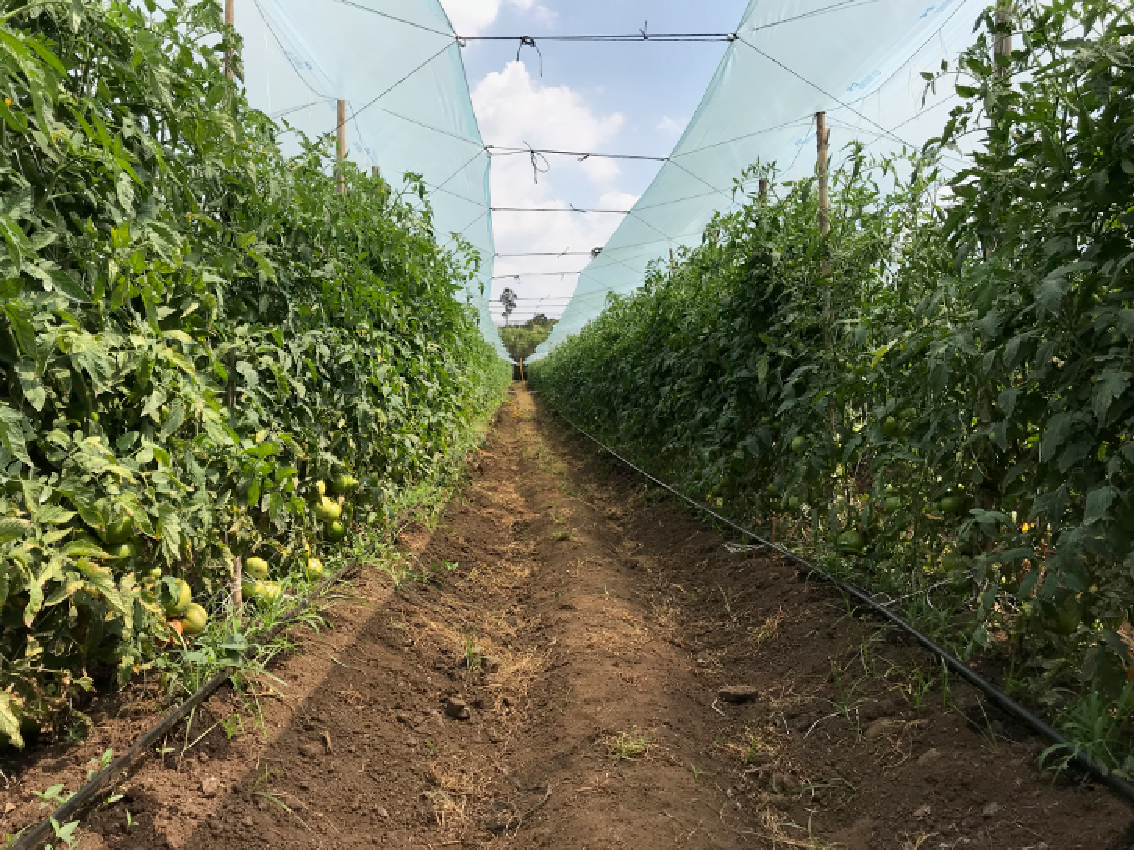
\includegraphics[width=100mm]{tomato_crop}
  \caption[Tomato crop]{Tomato crop in Costa Rica.}
  \label{fig:tomato_crop}
\end{figure}

\section{Video considerations}

\begin{itemize}
 \item The video resolution must be 1920x1080 pixels.
 \item Make use of a video stabilizer like a Gimbal. (For example the DJI Osmo Mobile 2)
 \item The video must be recorded in color.
 \item The duration of the video will depend on the length of the groove.
 \item The distance of the chamber from the plants should be approximately 1.5 meters.
 \item The video should cover the entire structure of the plant, from its base to the highest branches. If it is not possible to cover the entire plant in the same video, it will be done in different videos, covering in one of them the upper part of the plant and in another the lower part.
 \item Use the camera of a cell phone with Android or iOS operating systems.
 \item Use a mobile application that is capable of controlling the cell phone's front camera. Suggested applications: Filmic Pro.
 \item Utilizar una tarjeta de calibración de color previo a realizar los videos.
\end{itemize}

\section{Instructions for capturing the video}

As mentioned earlier, the videos cover each groove that confirms tomato plantations. Below are instructions to correctly capture the videos:

\begin{figure}[htb]
  \centering
  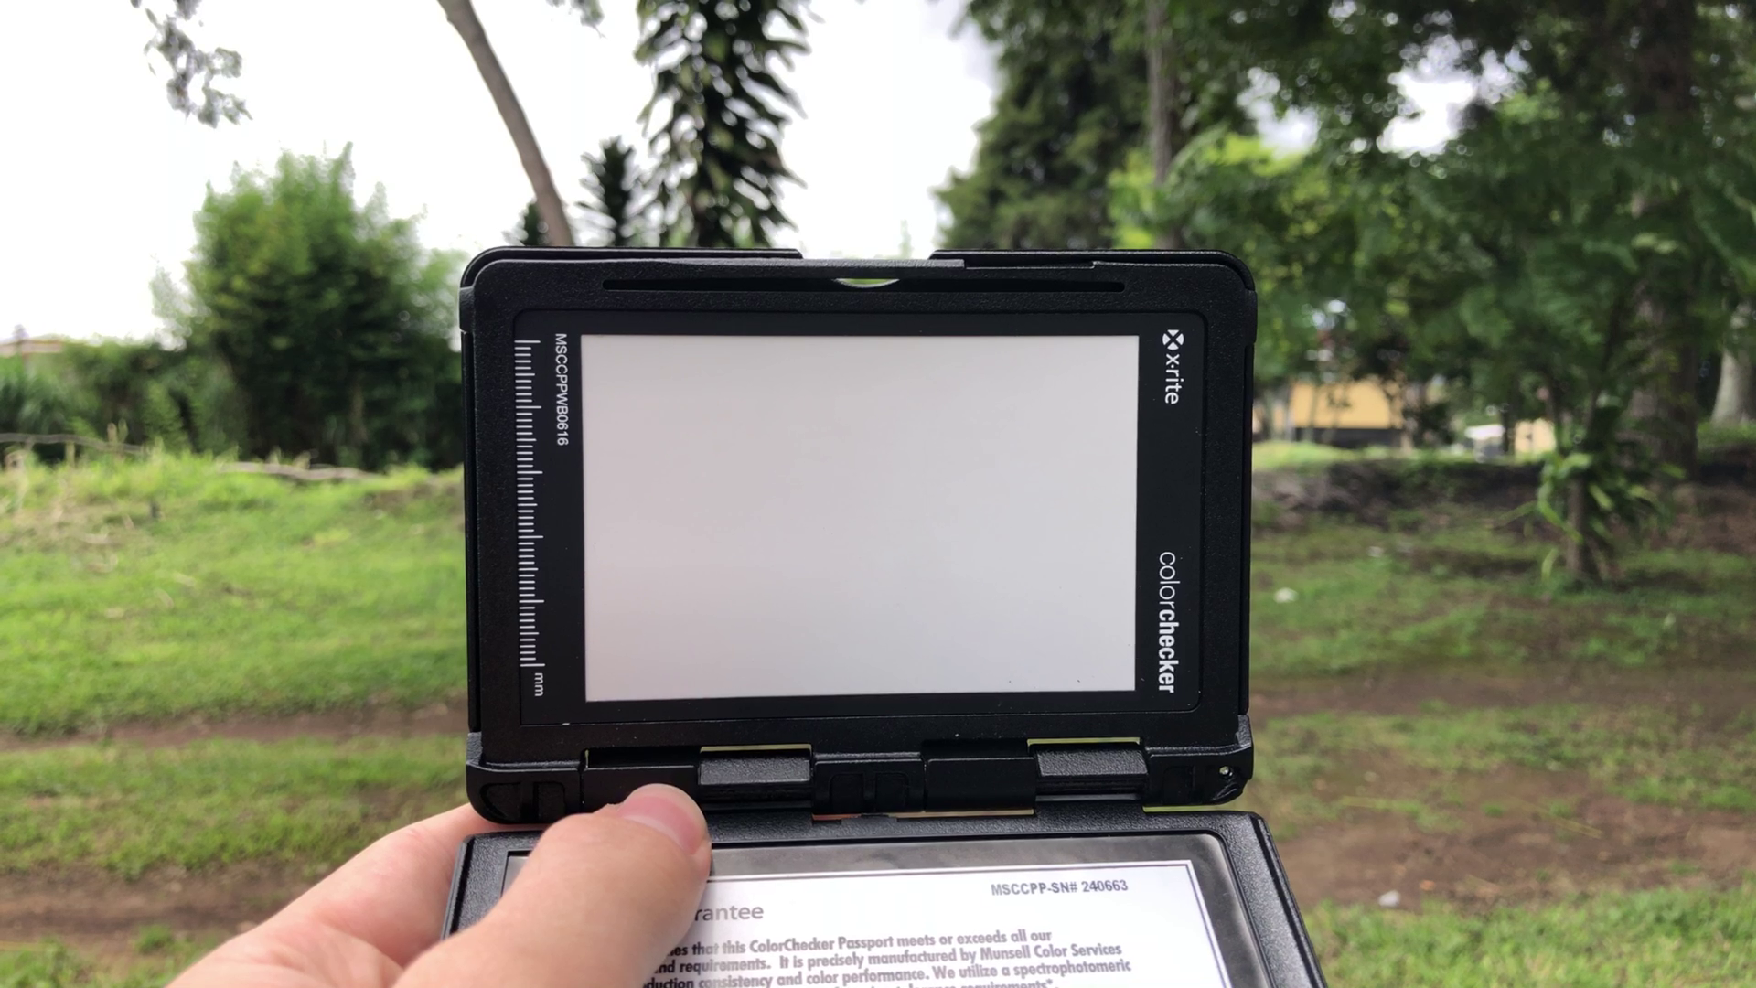
\includegraphics[width=100mm]{protocol2}
  \caption[Color calibration]{Colo checker gray card.}
  \label{fig:color_calibration}
\end{figure}

\subsection{Color calibration}

Using a gray scale calibration card, the camera's white balance should be adjusted as follows.

\begin{enumerate}
 \item Enter to the Filmic Pro application.
 \item Position the calibration card in front of the camera and zoom in to focus on the card only.
 \item Go to the camera settings and select the section related to white balance.
 \item Select the option to perform an automatic white balance.
 \item Wait a moment for the camera's white balance to be automatically adjusted and then select the option to set the white balance.
 \item It is important to mention that this process must be carried out in the place where the capture is intended and it is also recommended to repeat the steps every 30 minutes, to anticipate possible changes in the lighting that the place presents.
\end{enumerate}

\begin{figure}[H]
\begin{minipage}{\linewidth}
  \centering
  \begin{tabular}{ccc}
  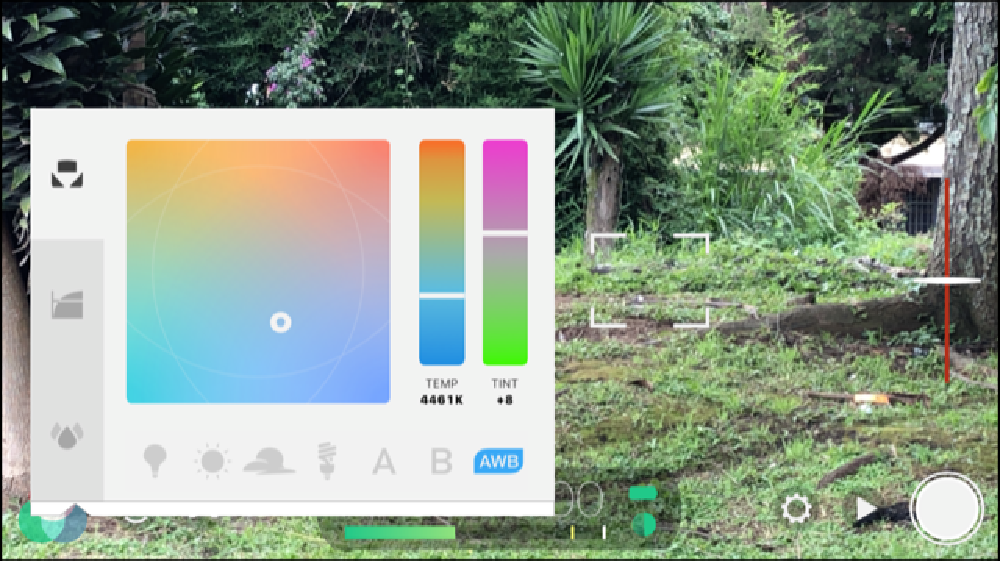
\includegraphics[width=.40\linewidth]{protocol4}
    & 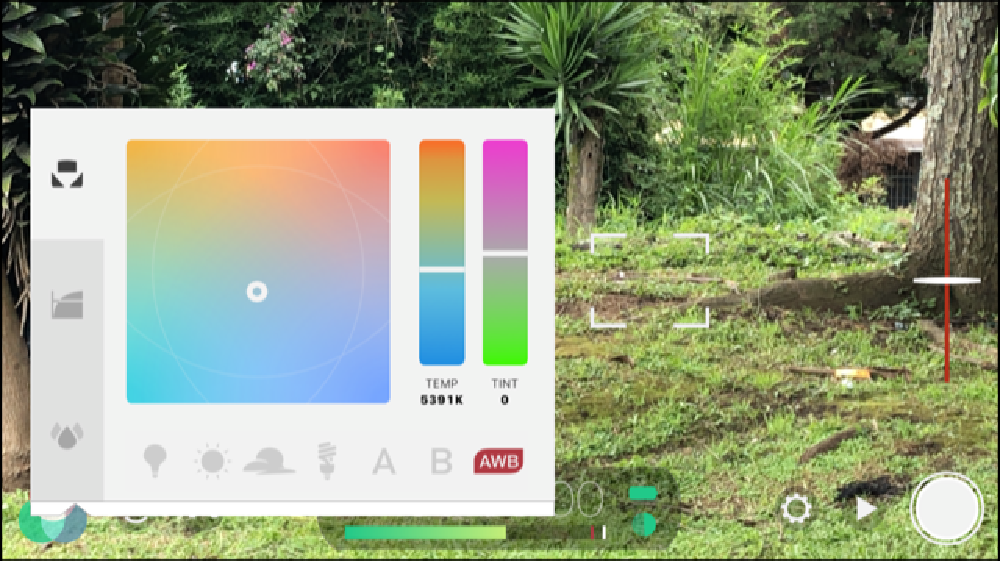
\includegraphics[width=.40\linewidth]{protocol5} \\
  (a) & (b) 
  \end{tabular}
  \end{minipage}
\caption[Whitebalance configuration]{Whitebalance configuration: In a) the automatic white balance is displayed and in b) the fixed white balance.}
\label{fig:whitebalance}
\end{figure}

\subsection{Proper use of the gimbal}

The following are some recommendations for optimal use of the gimbal.

\begin{enumerate}
 \item Make use of a tripod that allows you to make a gimbal grip with both hands.
 \item Tilt the device slightly forward in order to have greater stability during video capture.
 \item Make slow and constant movements. The suggested way of walking with the gimbal is to slightly bend the knees to have greater cushioning of the steps and avoid sudden movements of the camera.
\end{enumerate}

\subsection{Pre-capture application settings}

In order to avoid as much as possible the effect of blurring that can cause the taking of a moving video, it is recommended to set the frame rate of the application to 120 FPS and thus achieve a slow motion effect.



  %----------------------------------------------------------------------------
  \backmatter
  %----------------------------------------------------------------------------

  \printindex                % insert index into document. Don't forget to call
                             % "makeindex filename" first.
\end{document}
